% ============================================================================
%  Problems: รูปสองมิติ (2D Shapes)
%  Ordered from easy (basic) → intermediate.
%  Shared by exercise.tex and answer-key.tex
% ============================================================================

% --- Part 1: พื้นฐาน (Basic) ---
\examsection{ตอนที่ 1: พื้นฐาน — สูตรพื้นที่และเส้นรอบรูป}

\problem{
  สี่เหลี่ยมจัตุรัสมีด้านยาว $9$ ซม. จงหาพื้นที่และเส้นรอบรูป
}{
  พื้นที่ $= 9^2 = 81$ ตร.ซม.

  เส้นรอบรูป $= 4 \times 9 = 36$ ซม.
}

\problem{
  สี่เหลี่ยมผืนผ้ามีความกว้าง $5$ ซม. และความยาว $12$ ซม.
  จงหาพื้นที่และเส้นรอบรูป
}{
  พื้นที่ $= 5 \times 12 = 60$ ตร.ซม.

  เส้นรอบรูป $= 2(5 + 12) = 34$ ซม.
}

\problem{
  สามเหลี่ยมมีฐานยาว $10$ ซม. และสูง $6$ ซม. จงหาพื้นที่
}{
  $A = \dfrac{1}{2} \times 10 \times 6 = 30$ ตร.ซม.
}

\problem{
  สี่เหลี่ยมด้านขนานมีฐานยาว $8$ ซม. และสูง $5$ ซม.
  จงหาพื้นที่
}{
  $A = 8 \times 5 = 40$ ตร.ซม.
}

% --- Part 2: การประยุกต์ (Intermediate) ---
\examsection{ตอนที่ 2: การประยุกต์ — สี่เหลี่ยมและรูปหลายเหลี่ยม}

\problem{
  สี่เหลี่ยมขนมเปียกปูนมีเส้นทแยงมุมยาว $12$ และ $16$ ซม.
  จงหาพื้นที่
}{
  $A = \dfrac{1}{2} \times 12 \times 16 = 96$ ตร.ซม.
}

\problem{
  สี่เหลี่ยมคางหมูมีด้านคู่ขนานยาว $7$ และ $13$ ซม. สูง $8$ ซม.
  จงหาพื้นที่
}{
  $A = \dfrac{1}{2}(7 + 13) \times 8
      = \dfrac{1}{2} \times 20 \times 8 = 80$ ตร.ซม.
}

\problem{
  รูปหกเหลี่ยมปกติมีขนาดมุมภายในแต่ละมุมกี่องศา?
}{
  มุมภายใน $= \dfrac{(6-2) \times 180^\circ}{6}
               = \dfrac{720^\circ}{6} = 120^\circ$
}

\problem{
  รูปหลายเหลี่ยมปกติรูปหนึ่งมีมุมภายในแต่ละมุม $= 135^\circ$
  จงหาจำนวนด้านของรูปหลายเหลี่ยมนี้
}{
  $\dfrac{(n-2) \times 180^\circ}{n} = 135^\circ$

  $180n - 360 = 135n \;\Rightarrow\; 45n = 360 \;\Rightarrow\; n = 8$
}

\problem{
  จงหาจำนวนเส้นทแยงมุมของรูปห้าเหลี่ยมนูน
}{
  $\dfrac{5(5-3)}{2} = \dfrac{5 \times 2}{2} = 5$ เส้น
}

\problem{
  รูปหลายเหลี่ยมใดต่อไปนี้เป็นรูปหลายเหลี่ยมเว้า (concave)?
  \begin{itemize}
    \item[ก.] รูปที่มีมุมภายในทุกมุมน้อยกว่า $180^\circ$
    \item[ข.] รูปที่มีมุมภายในมุมหนึ่งเป็น $210^\circ$
    \item[ค.] รูปสี่เหลี่ยมจัตุรัส
  \end{itemize}
}{
  \textbf{ข.} รูปที่มีมุมภายใน $210^\circ > 180^\circ$ (มุมกลับ)
  ดังนั้นเป็นรูปหลายเหลี่ยมเว้า

  ก. และ ค. เป็นรูปหลายเหลี่ยมนูน
}

% --- Part 3: ระดับ สอวน. (POSN Level) ---
\examsection{ตอนที่ 3: ระดับข้อสอบ สอวน.}

\problem{
  (ข้อสอบจริงปี 67 ข้อ 19) ให้รูปสี่เหลี่ยมด้านขนาน ABCD มาตามรูป และให้ AB ยาว 30 ซม. ถ้าลากเส้น EA (ต่อเชื่อมจากเส้น AB) และเส้น EF เพิ่ม โดยจุด F เป็นจุดบนเส้น AD และ จุด E เป็นมุมฉาก ให้ FD ยาว 15 ซม. EA ยาว 4 ซม. EF ยาว 3 ซม. จงหาว่า พื้นที่สี่เหลี่ยม ABCD มีค่าเท่าใด (Hint: ใช้เรื่องสามเหลี่ยมคล้าย)
  \begin{center}
    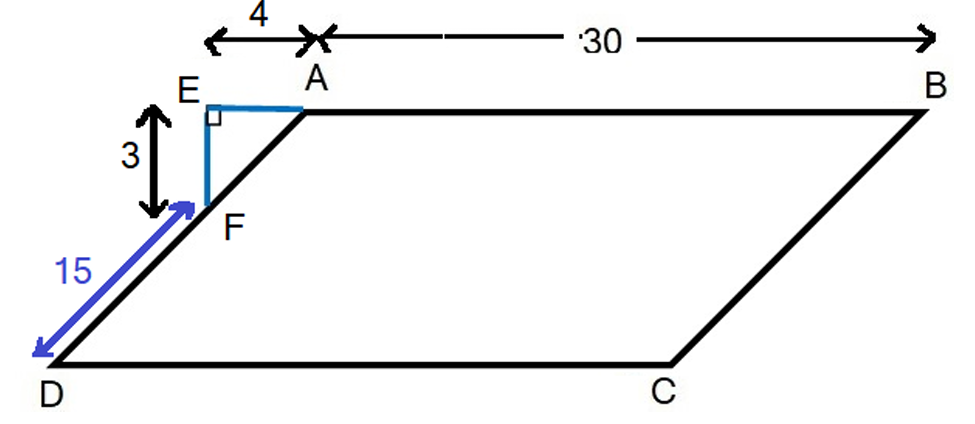
\includegraphics[width=0.5\textwidth]{images/geometry-2d-01.png}
  \end{center}
}{
  $360$ ตร.ซม.
}

\problem{
  (ข้อสอบจริงปี 67 ข้อ 29) จากรูปที่กำหนดให้อยากทราบว่าค่าผลรวมของมุม x และมุม y มีค่าเท่าไร 
  \begin{center}
    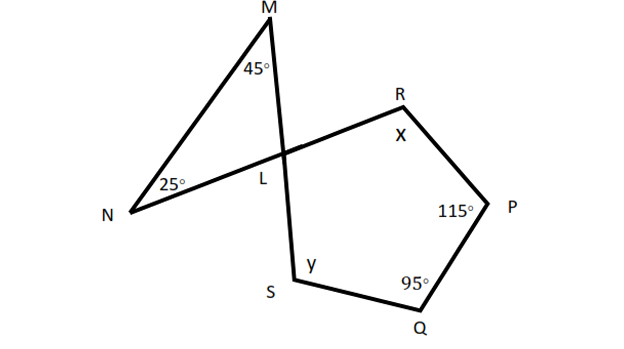
\includegraphics[width=0.5\textwidth]{images/geometry-2d-02.png}
  \end{center}
}{
  $220^\circ$
}